\documentclass[aspectratio=169]{beamer}

\usepackage[utf8]{inputenc}
\usetheme{Madrid}
\usecolortheme{beaver}

\usepackage{graphicx}
\graphicspath{ {./Resources/} }

\title{ConOps - Inverted Pendulum PID Controller}       % Title
\author{Austin, Joe, Matt, Kathryn}                     % Team members
\institute{SNHU/CETA}                                   % Institute
\logo{
\includegraphics[height=0.8cm]{../../AJMK_Logo}}  % Our Logo

\begin{document}

\frame{\titlepage} % Draw the title page


\begin{frame}                     % A frame/page/slide
    \frametitle{Stakeholders}     % Title

    \begin{block}{Stakeholders}   % Blocks are just nice places to encapsulate other things
        \begin{itemize}           % Like this list!
            \item Education (higher)
            \item Education (lower)
            \item Industrial training device
            \item Educational Toy Industry
        \end{itemize}
    \end{block}

    \begin{block}{Users}
        \begin{itemize}
            \item Professors
            \item Teachers
            \item Educators
            \item On-Boarding / Hiring of Software Engineers
        \end{itemize}
    \end{block}

\end{frame}


\begin{frame}
    \frametitle{System Description}

    We want a conveyor assembly controlled by a NEMA-17 motor, sliding on circular linear rods
    using harmonic osculations to bring the pendulum to a starting position, and then hold there
    using an embedded PID. The system will have three potentiometers, a TFT-screen, and a button on the user control panel. All encased in a transparent housing.

    \begin{block}{}
        The users will be able to modify the PID values on the fly using the potentiometers to learn and experiment
        with the concept of PID loops after the press of a button on the front of the user control panel.
    \end{block}

\end{frame}


\begin{frame}
    \frametitle{Operational Environment}

    Our demonstrator will be in a:
    \begin{itemize}
        \item High traffic environment
        \item Possibly dusty
        \item Indoors
        \item Powered on 24/7
    \end{itemize}

    We'll need to think about

    \begin{itemize}
        \item Wearing components (belts, sliders)
        \item Constant touching and interaction
        \item Low power/sleep mode
        \item Heat Cycles
    \end{itemize}

\end{frame}


\begin{frame}
    \frametitle{Support Environment}

    \begin{block}{COTS Parts}
        Our demonstrator will be made from as many COTS (Common Off The Shelf) parts
        as possible to ensure simple replacement.
        Some of the wearing will be the belt, the linear bearing, the fans may need replacement, power cord, the bearings may need to be lubed occasionally, and Loctite will need to be applied to screws to prevent them from backing out due to vibrations from the motor.
    \end{block}

    \begin{block}{Modularity}
        Our demonstrator will be made from modular sections and de-constructable segments
        to facilitate service and storage.
    \end{block}

    \begin{block}{Calibration}
        The pendulum will be self calibrating using gravity.
    \end{block}

\end{frame}


\begin{frame}
    \frametitle{Operating Modes}
    % Operating modes goes here

    \begin{itemize}
        \item Off mode: the state in which the system is powered down and or unplugged.
        \item Idle mode: a power saving mode in which fans are turned off; the TFT screen is turned off; and the motor controller, CPU, and power supply will be swapped to their internal lower power consumption mode.
        \item Spin-up mode: a custom control procedure that self initializes (swing the pendulum up into a ready state using harmonic oscillation.
        \item Demo PID mode: a build-in PID procedure with lock Kp, Ki, and Kd values to demonstrate how the inverse pendulum is properly balanced.
        \item User PID mode: a control structure in which the user can manipulate the Kp, Ki, and Kd constants to witness the effects of their changes on the stability of the pendulum.
    \end{itemize}

\end{frame}


\begin{frame}
    \frametitle{Use}
    The system will be serviceable and long-lasting. The system should be reliable and precise, and be able to operate often long periods of non-usage.
    \vspace{.5cm}
    We hope that our demonstrator may find semi-permanent use educating students and future
    engineers here and in market!

\end{frame}


\begin{frame}
    \frametitle{Risks}

    Some risks

    \begin{itemize}
        \item Pinch Points and swinging pendulum.
        \item [-] Capacitive e-stop technology as well as sound alerts when the system begins to move, and a transparent shield / cover to isolate the dynamic system.
        \item Failure in on duty.
        \item [-] Easily serviceable parts.
        \item Prevention of self destruction due to inexperienced or unknowing user.
        \item [-] Software locks, an e-stop switch, and a rubber bumper / mechanical hard stop.
        \item Electrical short
        \item [-] Have a fused power supply, and will follow IEC standards with proper grounding.
        \item Electrical heat
        \item [-] Embedded fans in the storage with plenty of holes for ventilation.
    \end{itemize}

\end{frame}

\begin{frame}
    \frametitle{Impact Considerations}

    \begin{block}{Social Impacts}
        \begin{itemize}
            \item PID will become a more widely understood control system, and students will be able to more efficiently tune their PID loops.
            \item The ease of education into control systems using the product may sway more interest more of he younger generation into the engineering fields.
            \item Higher education could give the system without the embedded PID loop and create a project in which students must start form scratch to balance the pendulum.

        \end{itemize}
    \end{block}

    \begin{block}{Environmental Impacts}
        \begin{itemize}
            \item Create a larger current draw on the environment.
            \item Portions of the electronics have rare-earth metals that the Earth has a limited supply of.
            \item The system takes up physical space wherever it is installed, and as new iterations are created, the system may be thrown out.
        \end{itemize}
    \end{block}





\end{frame}

\begin{frame}
    \frametitle{Initial Renders (1/2)}

    \begin{columns}                         % You can use a columnn (or row) to split the screen
        \begin{column}{0.48\textwidth}
            \begin{block}{Initial Sketch}
                We hope that our final design may look something like this!
            \end{block}
        \end{column}
        \begin{column}{0.48\textwidth}
            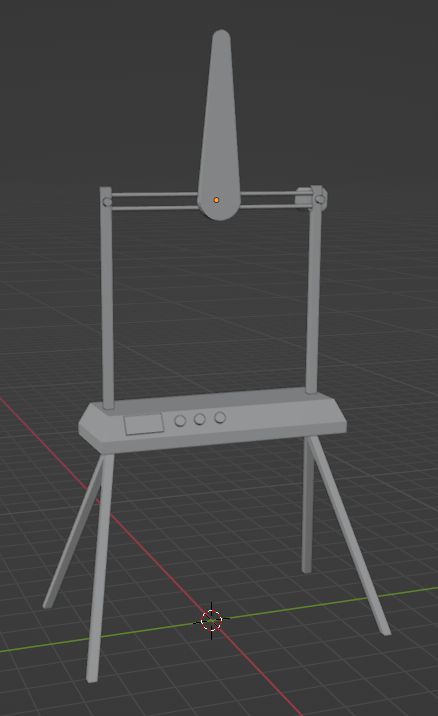
\includegraphics[height=7cm]{Full}
        \end{column}
    \end{columns}

\end{frame}


\begin{frame}
    \frametitle{Initial Renders (2/2)}

    \begin{columns}
        \begin{column}{0.48\textwidth}
            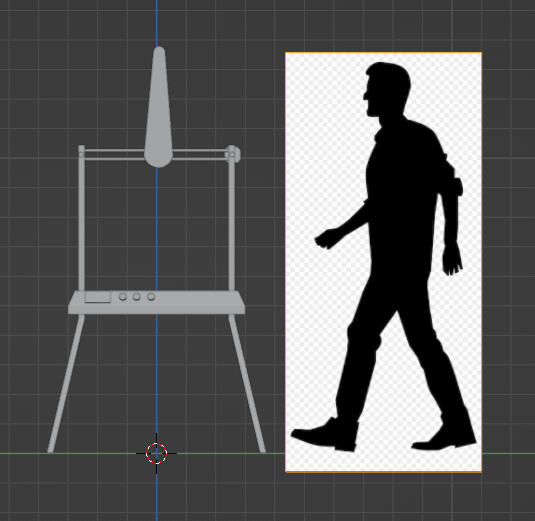
\includegraphics[width=5cm]{Scale}
        \end{column}
        \begin{column}{0.48\textwidth}
            \begin{block}{Initial Sketch}
                We'd like it to stand about this tall (left) to facilitate easy access
                and usage. With a simple and minimalist visible drivetrain (Below).
            \end{block}
            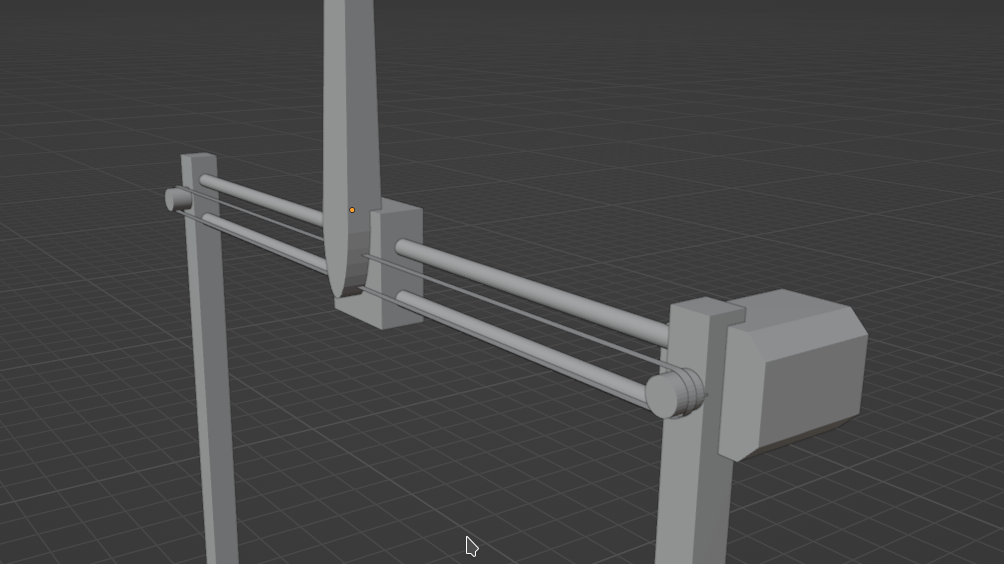
\includegraphics[width=5cm]{UpperAssy}
        \end{column}
    \end{columns}

\end{frame}

\begin{frame}
    \frametitle{Initial Sketches (1/2)}

    \begin{columns}
        \begin{column}{0.48\textwidth}
            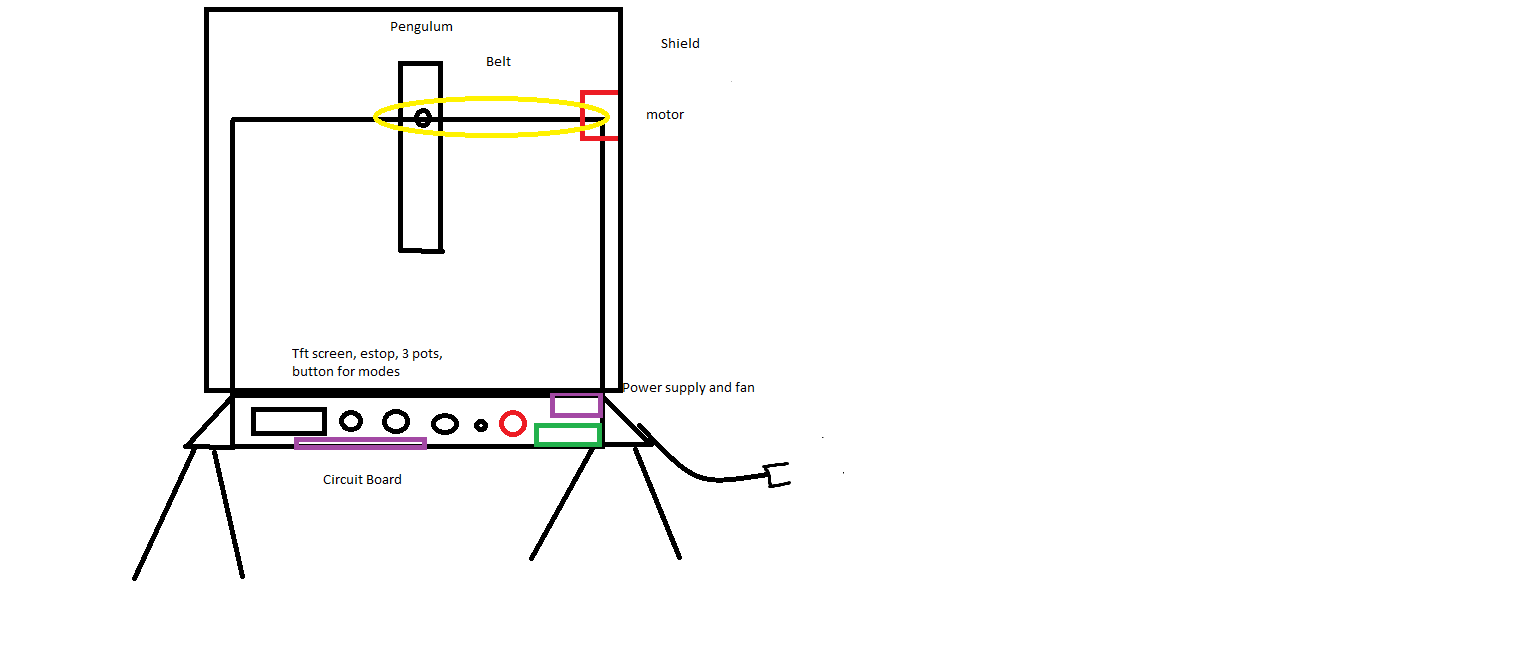
\includegraphics[width=7cm]{../../Notes/Sketches/Basic Mock-Up Sketch.png}
        \end{column}
        \begin{column}{0.48\textwidth}
            \begin{block}{Initial Sketch}
                Sketch design
            \end{block}
        \end{column}
    \end{columns}
\end{frame}

\begin{frame}
    \frametitle{Initial Sketches (2/2)}

    \begin{columns}
        \begin{column}{0.48\textwidth}
            \begin{block}{Initial Sketch}
                Stackup design for the pendulum bearing.
            \end{block}
        \end{column}
        \begin{column}{0.48\textwidth}
            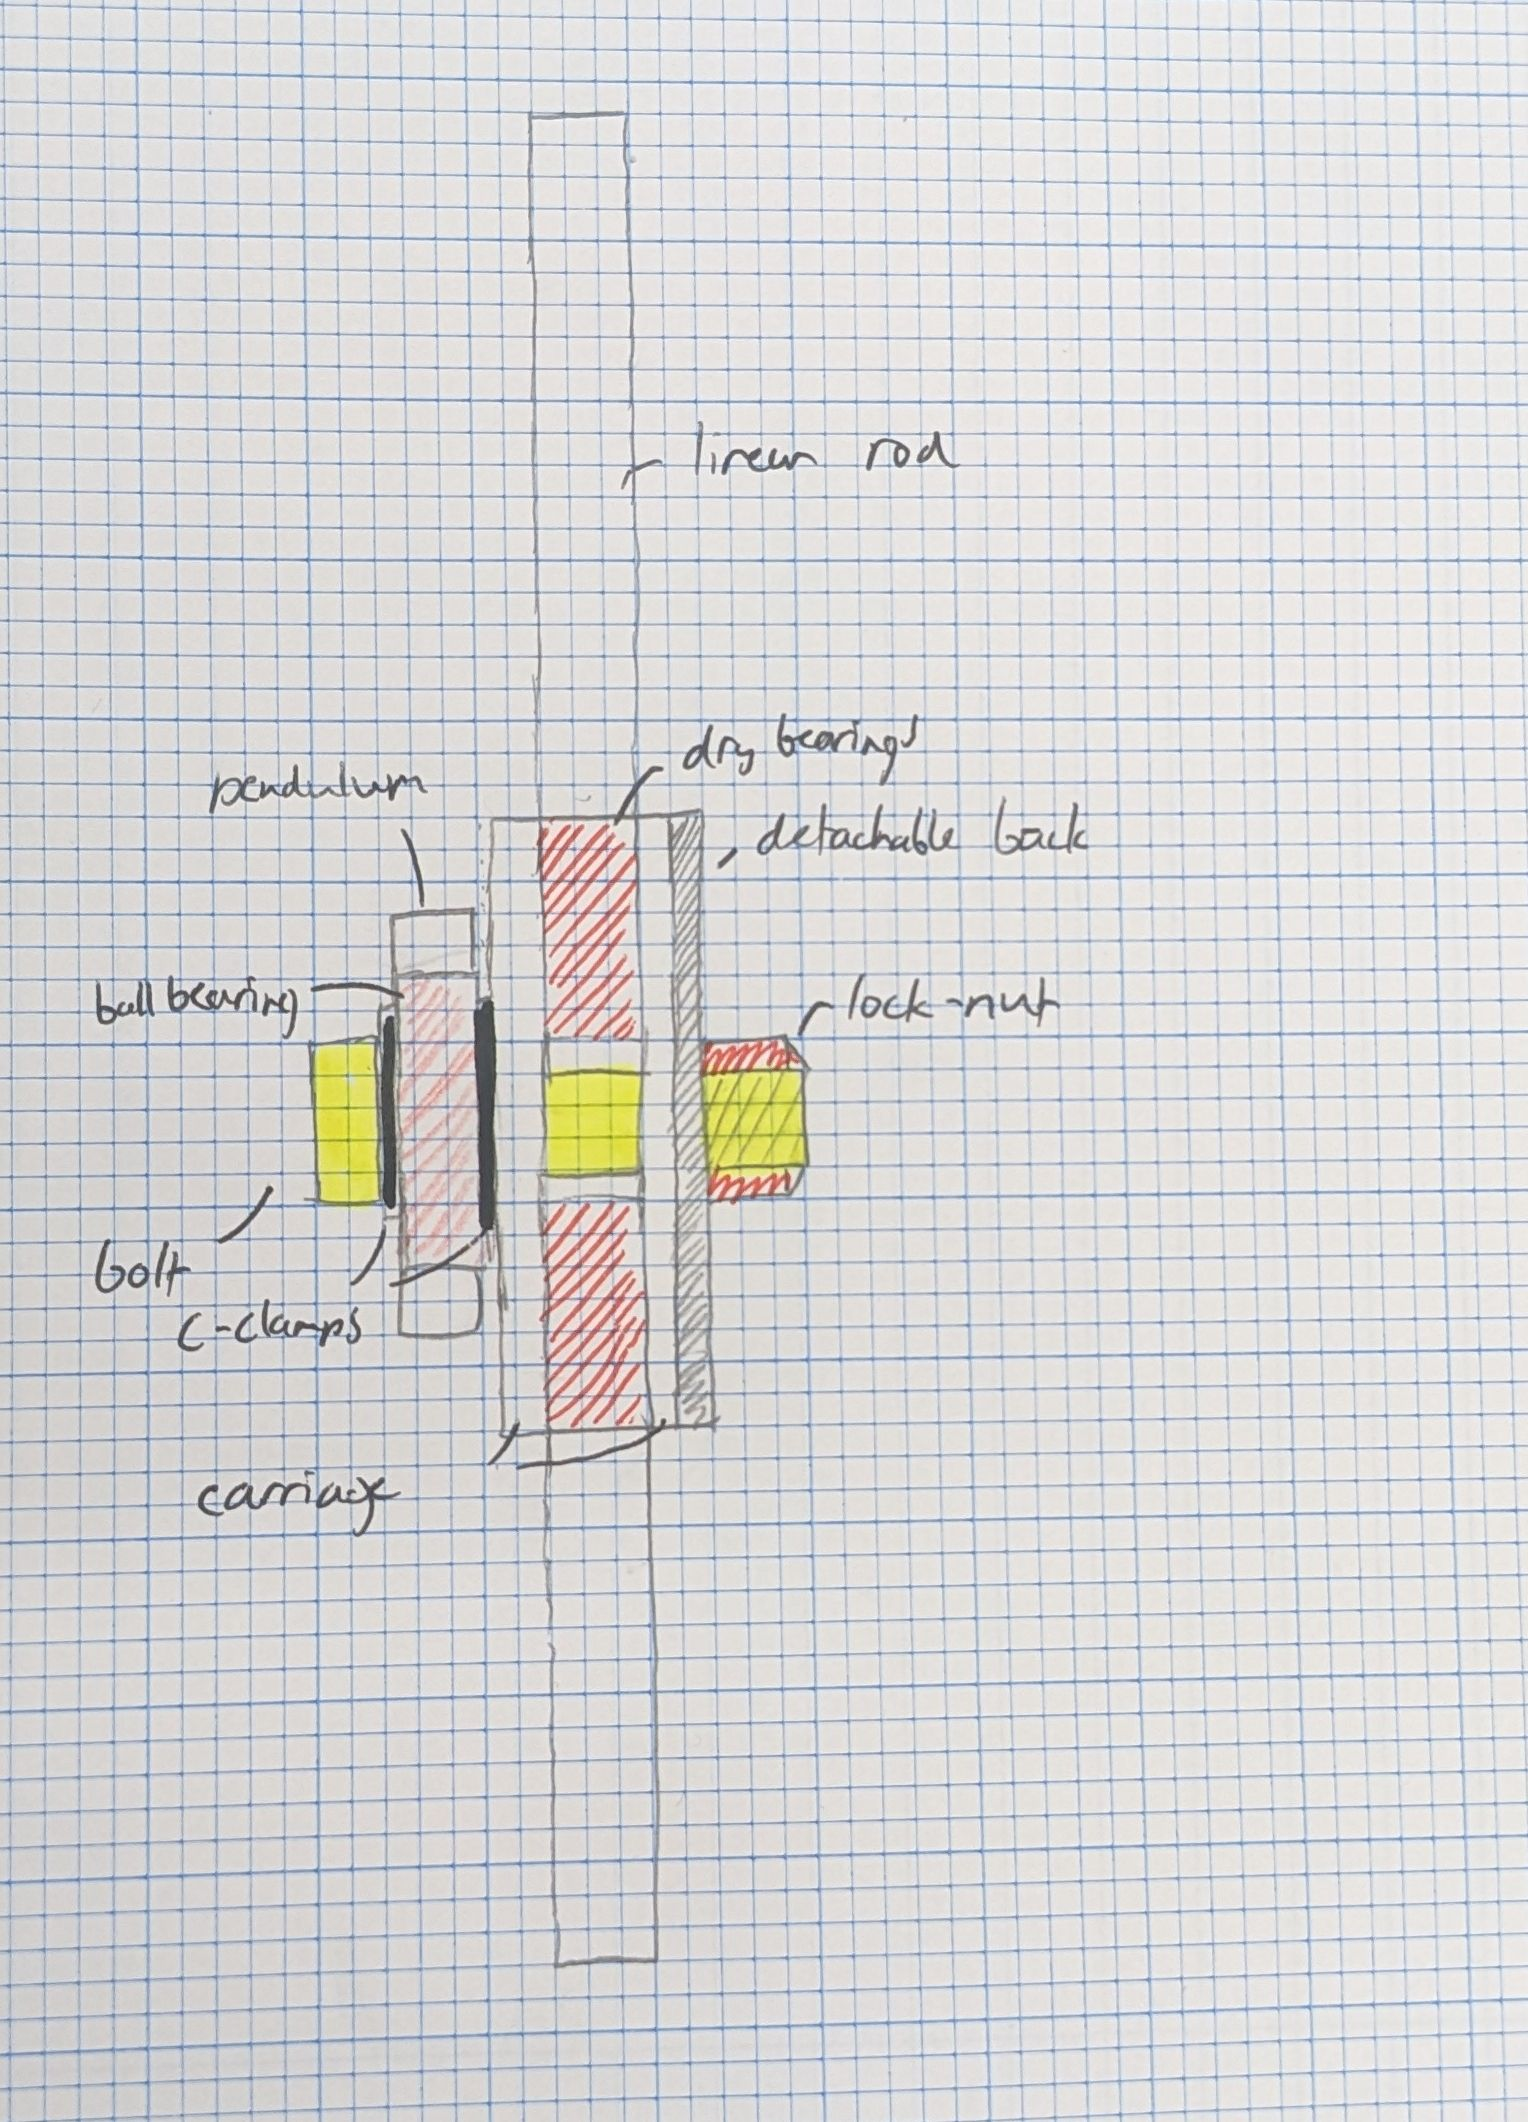
\includegraphics[height=7cm]{../../Notes/Sketches/BearingStackup.jpg}
        \end{column}
    \end{columns}
\end{frame}


\begin{frame}
    \frametitle{End}

    \begin{center}
        
\includegraphics[height=1.5cm]{../../AJMK_Logo}
    \end{center}


    \begin{block}{}
        \begin{center}
            \Huge Questions and Comments?
        \end{center}
    \end{block}

    \begin{center}
        Find the source code for this document, and the rest of our designs, firmware, hardware
        and notes on GitHub!

        
\includegraphics[height=2cm]{github_qr}
    \end{center}

\end{frame}


\end{document}
